\documentclass[12pt]{report}
\usepackage{graphicx}     %Note graphics<graphicx<epsfig
\usepackage[table,xcdraw, dvipsnames]{xcolor}
\usepackage{hyperref} %written by Sebastian Rahtz
%\usepackage{subeqn}    %allows equations 1a, 1b
%\usepackage{subfig}    %allows figures 1a, 1b
\usepackage{amsmath}
\usepackage{amssymb}
\usepackage{xurl}
\usepackage{bbm}%for indicator function
%\bibliographystyle{alpha}
\usepackage{floatrow}
\usepackage[normalem]{ulem}


\usepackage{tocloft}

% Adjust number widths
\setlength{\cftchapnumwidth}{2em}
\setlength{\cftsecnumwidth}{3.2em}
\setlength{\cftsubsecnumwidth}{3.5em}

\usepackage[toc,page]{appendix}
\usepackage[nottoc]{tocbibind}

\usepackage[color,matrix,frame,arrow,curve]{xy}
\usepackage[shortlabels]{enumitem}
\usepackage{array}
\usepackage{pdflscape}
\usepackage{multicol, multirow}
\usepackage{ctable}
\usepackage{dirtree}
\usepackage{subfig}
\usepackage{longtable}

%\usepackage{fdsymbol}
%\usepackage{animate}% play animation

\usepackage[vlined,ruled]{algorithm2e}
\newcommand{\mycommfont}[1]{\small\ttfamily\textcolor{blue}{#1}}
\SetCommentSty{mycommfont}

%highlighting
\usepackage{mdframed}

\usepackage[makeroom]{cancel}

\usepackage{pdfpages}
\usepackage{hyperxmp}

% this escapes the underscore in text
%\usepackage[T1]{fontenc}
%\usepackage{underscore}

\paperheight=11in
\topmargin=0in
\headheight=0in
\headsep=0in
\topskip=0in
\textheight=8.5in
\footskip=.5in


\paperwidth=8.5in
\oddsidemargin=.25in
\evensidemargin=.25in
\textwidth=6.0in
\parindent=.5in

\newcommand{\chapquote}[3]{\begin{quotation} \textit{#1} \end{quotation} \begin{flushright} - #2, \textit{#3}\end{flushright} }

\newtheorem{claim}{Claim}
\newcommand{\proof}[0]{{\bf proof:} }
\newcommand{\qed}[0]{\quad\newline \noindent{\bf QED }}

\newcommand{\upto}[0]{-}
\newcommand{\XT}[2]{{\substack{#1\\#2}}}

\newcommand{\bra}[1]{\langle#1|}
\newcommand{\ket}[1]{|#1\rangle}
\newcommand{\av}[1]{\left\langle#1\right\rangle}
\newcommand{\pder}[2]{\frac{\partial#1}{\partial#2}}
\newcommand{\der}[2]{\frac{d#1}{d#2}}
\newcommand{\tr}[0]{{\rm tr }}
\newcommand{\beq}{\begin{equation}}
\newcommand{\eeq}{\end{equation}}
\newcommand{\bsub}{\begin{subequations}}
	\newcommand{\esub}{\end{subequations}}
\newcommand{\beqa}{\begin{eqnarray}}
\newcommand{\eeqa}{\end{eqnarray}}
\newcommand{\rarrow}[0]{\rightarrow}
\newcommand{\larrow}[0]{\leftarrow}
\newcommand{\uarrow}[0]{\uparrow}
\newcommand{\darrow}[0]{\downarrow}
\newcommand{\Rarrow}[0]{\Rightarrow}
\newcommand{\nRarrow}[0]{\nRightarrow}
\newcommand{\Larrow}[0]{\Leftarrow}
\newcommand{\nLarrow}[0]{\nLeftarrow}
\newcommand{\ul}[1]{\uline{#1}}
\newcommand{\ol}[1]{\overline{#1}}
\newcommand{\CC}[0]{{ \mathbb{C}} }
\newcommand{\EE}[0]{{ \mathbb{E}} }
\newcommand{\NNN}[0]{ {\mathbb{N}}} %\NN already defined
\newcommand{\RR}[0]{{ \mathbb{R}} }
\newcommand{\WW}[0]{ {\mathbb{W}}}
\newcommand{\XX}[0]{{ \mathbb{X}} }
\newcommand{\ZZ}[0]{ {\mathbb{Z}}}

\newcommand{\ground}{{}_{\stackrel{\stackrel{\displaystyle{\bot}}{-}}{.}}}
\newcommand{\norm}[1]{\parallel#1\parallel}
\newcommand{\eqdef}[0]{\;\;\stackrel{\text{def}}{=}\;\;}

\newcommand{\heavy}[0]{\mathbf{H}}

\newcommand{\rva}[0]{{\ul{a}}}
\newcommand{\rvb}[0]{{\ul{b}}}
\newcommand{\rvc}[0]{{\ul{c}}}
\newcommand{\rvd}[0]{{\ul{d}}}
\newcommand{\rve}[0]{{\ul{e}}}
\newcommand{\rvf}[0]{{\ul{f}}}
\newcommand{\rvg}[0]{{\ul{g}}}
\newcommand{\rvh}[0]{{\ul{h}}}
\newcommand{\rvi}[0]{{\ul{i}}}
\newcommand{\rvj}[0]{{\ul{j}}}
\newcommand{\rvk}[0]{{\ul{k}}}
\newcommand{\rvl}[0]{{\ul{l}}}
\newcommand{\rvll}[0]{{\ul{\ell}}}
\newcommand{\rvm}[0]{{\ul{m}}}
\newcommand{\rvn}[0]{{\ul{n}}}
\newcommand{\rvo}[0]{{\ul{o}}}
\newcommand{\rvp}[0]{{\ul{p}}}
\newcommand{\rvq}[0]{{\ul{q}}}
\newcommand{\rvr}[0]{{\ul{r}}}
\newcommand{\rvs}[0]{{\ul{s}}}
\newcommand{\rvt}[0]{{\ul{t}}}
\newcommand{\rvu}[0]{{\ul{u}}}
\newcommand{\rvv}[0]{{\ul{v}}}
\newcommand{\rvw}[0]{{\ul{w}}}
\newcommand{\rvx}[0]{{\ul{x}}}
\newcommand{\rvy}[0]{{\ul{y}}}
\newcommand{\rvz}[0]{{\ul{z}}}


\newcommand{\rvA}[0]{{\ul{A}}}
\newcommand{\rvB}[0]{{\ul{B}}}
\newcommand{\rvC}[0]{{\ul{C}}}
\newcommand{\rvD}[0]{{\ul{D}}}
\newcommand{\rvE}[0]{{\ul{E}}}
\newcommand{\rvF}[0]{{\ul{F}}}
\newcommand{\rvG}[0]{{\ul{G}}}
\newcommand{\rvH}[0]{{\ul{H}}}
\newcommand{\rvI}[0]{{\ul{I}}}
\newcommand{\rvJ}[0]{{\ul{J}}}
\newcommand{\rvK}[0]{{\ul{K}}}
\newcommand{\rvL}[0]{{\ul{L}}}
\newcommand{\rvM}[0]{{\ul{M}}}
\newcommand{\rvN}[0]{{\ul{N}}}
\newcommand{\rvO}[0]{{\ul{O}}}
\newcommand{\rvP}[0]{{\ul{P}}}
\newcommand{\rvQ}[0]{{\ul{Q}}}
\newcommand{\rvR}[0]{{\ul{R}}}
\newcommand{\rvS}[0]{{\ul{S}}}
\newcommand{\rvT}[0]{{\ul{T}}}
\newcommand{\rvU}[0]{{\ul{U}}}
\newcommand{\rvV}[0]{{\ul{V}}}
\newcommand{\rvW}[0]{{\ul{W}}}
\newcommand{\rvX}[0]{{\ul{X}}}
\newcommand{\rvY}[0]{{\ul{Y}}}
\newcommand{\rvZ}[0]{{\ul{Z}}}

\newcommand{\rvbeta}[0]{{\ul{\beta}}}
\newcommand{\rvxi}[0]{{\ul{\xi}}}
\newcommand{\rvzeta}[0]{{\ul{\zeta}}}
\newcommand{\rvtheta}[0]{{\ul{\theta}}}
\newcommand{\rvmu}[0]{{\ul{\mu}}}
\newcommand{\rvsig}[0]{{\ul{\sigma}}}
\newcommand{\rvDel}[0]{{\ul{\Delta}}}
\newcommand{\rvtau}[0]{{\ul{\tau}}}

\newcommand{\cala}[0]{{\cal A}}
\newcommand{\calb}[0]{{\cal B}}
\newcommand{\calc}[0]{{\cal C}}
\newcommand{\cald}[0]{{\cal D}}
\newcommand{\cale}[0]{{\cal E}}
\newcommand{\calf}[0]{{\cal F}}
\newcommand{\calg}[0]{{\cal G}}
\newcommand{\calh}[0]{{\cal H}}
\newcommand{\cali}[0]{{\cal I}}
\newcommand{\calk}[0]{{\cal K}}
\newcommand{\call}[0]{{\cal L}}
\newcommand{\calm}[0]{{\cal M}}
\newcommand{\caln}[0]{{\cal N}}
\newcommand{\calo}[0]{{\cal O}}
\newcommand{\calp}[0]{{\cal P}}
\newcommand{\calq}[0]{{\cal Q}}
\newcommand{\calr}[0]{{\cal R}}
\newcommand{\cals}[0]{{\cal S}}
\newcommand{\calt}[0]{{\cal T}}
\newcommand{\calu}[0]{{\cal U}}
\newcommand{\calv}[0]{{\cal V}}
\newcommand{\calw}[0]{{\cal W}}
\newcommand{\calx}[0]{{\cal X}}
\newcommand{\caly}[0]{{\cal Y}}
\newcommand{\calz}[0]{{\cal Z}}

%\newcommand{\diamante}[1]{\Big\langle#1\Big\rangle}
\newcommand{\diamante}[1]{*++[F=]{#1}}
%\newcommand{\corchete}[1]{\Big\{#1\Big\}}
\newcommand{\corchete}[1]{#1}
\newcommand{\cuadro}[1]{*++[F]{#1}}

\newcommand{\Pmat}[4]{\calp\left[
\begin{array}{cc}#1&#2\\#3&#4
\end{array}\right]}

%\newcommand{\PN}[0]{PN^{0,0}_{1,1}}
%\newcommand{\PS}[0]{PS^{1,1}_{0,0}}
\newcommand{\PN}[0]{PN}
\newcommand{\PS}[0]{PS}

\newcommand{\lam}[0]{\lambda}
\newcommand{\Lam}[0]{\Lambda}
\newcommand{\alp}[0]{\alpha}
\newcommand{\eps}[0]{\epsilon}
\newcommand{\s}[0]{\sigma}
\newcommand{\su}[0]{{\Sigma}}

\newcommand{\pp}[0]{\mathbb{P}}
\newcommand{\dbm}[0]{{
		[1,\partial_{b},\partial_{m}]
}}

\newcommand{\dg}[0]{{[1, \partial_{\theta_G}]}}
\newcommand{\dd}[0]{{[1, \partial_{\theta_D}]}}
\newcommand{\dgd}[0]{{[1, \partial_{\theta_G}, \partial_{\theta_D}]}}

\newcommand{\veca}[0]{{\vec{a}}}
\newcommand{\vecb}[0]{{\vec{b}}}
\newcommand{\vecc}[0]{{\vec{c}}}
\newcommand{\vecd}[0]{{\vec{d}}}
\newcommand{\vecf}[0]{{\vec{f}}}
\newcommand{\vech}[0]{{\vec{h}}}
\newcommand{\vecr}[0]{{\vec{r}}}
\newcommand{\vecs}[0]{{\vec{s}}}
\newcommand{\vecu}[0]{{\vec{u}}}
\newcommand{\vecx}[0]{{\vec{x}}}
\newcommand{\vecy}[0]{{\vec{y}}}
\newcommand{\vechy}[0]{{\vec{\haty}}}
\newcommand{\vtheta}[0]{{\vec{\theta}}}

\newcommand{\haty}[0]{{\widehat{y}}}
\newcommand{\hatx}[0]{{\widehat{x}}}
\newcommand{\hata}[0]{{\widehat{a}}}
\newcommand{\hatr}[0]{{\widehat{r}}}


\newcommand{\cond}[0]{{\:\mathbf{|}\:}}
\newcommand{\mymathbf}[1]{#1}

\newcommand{\ranvec}[1]{\ul{\vec{#1}}}
\newcommand{\indi}[0]{\mathbbm{1}}
\newcommand{\smoid}[0]{{\rm smoid}}
\newcommand{\lodds}[0]{{\rm lodds}}
\newcommand{\expit}[0]{{\rm expit}}
\newcommand{\logit}[0]{{\rm logit}}
\newcommand{\sign}[0]{{\rm sign}}

\renewcommand{\labelitemii}{$\bullet$}

\newcommand{\HAT}[1]{{\widehat{#1}}}
\newcommand{\TIL}[1]{{\widetilde{#1}}}
\newcommand{\tild}[0]{{\TIL{d}}}
\newcommand{\tile}[0]{{\TIL{e}}}
\newcommand{\tilg}[0]{{\TIL{g}}}
\newcommand{\tilu}[0]{{\TIL{u}}}
\newcommand{\tilx}[0]{{\TIL{x}}}
\newcommand{\tilP}[0]{{\TIL{P}}}
\newcommand{\tilPT}[0]{{\TIL{P}_\theta}}

\newcommand{\maparrow}[1]
{\xymatrix{\ar[r]_{#1}&}}


\newcommand{\ucalm}[0]{\ul{\calm}}

\newcommand{\bool}[0]{\{0,1\}}

\newcommand{\argmin}{\mathop{\mathrm{argmin}}\limits}
\newcommand{\argmax}{\mathop{\mathrm{argmax}}\limits}

\newcommand{\softmax}[0]{{\rm softmax}}

\newcommand{\A}[0]{\wedge}
\newcommand{\V}[0]{\vee}
\newcommand{\xor}{\oplus}
\newcommand{\bigA}[0]{\bigwedge}
\newcommand{\bigV}[0]{\bigvee}
\newcommand{\bigxor}{\bigoplus}


\newcommand{\rdart}[0]{\Rightarrow}
\newcommand{\ldart}[0]{\Leftarrow}
\newcommand{\rveps}[0]{\ul{\eps}}

\newcommand{\hatvar}[0]{\widehat{\sigma^2}}
\newcommand{\ptp}[0]{{(t)}}

\newcommand{\tseries}[1]{{\{#1\}_{\forall t}}}

\newcommand{\xbeta}[0]{X_\s^T\beta}
\newcommand{\xtau}[0]{X_\s^T\tau}

%arguments phi1, phi2, phi3, e
\newcommand{\rbd}[4]{
\xymatrix@-1.3pc{
&#1\ar[d]&&#2\ar[d]
\\
&\rvx_1\ar[rr]
&&
\rvx_2
\ar `r[rd][rd]
\\
0\ar`u[u][ru]
\ar`d[dr][rrd]
&&&&\rvA\ar[r]&#4
\\
&&
\rvx_3
\ar `r[rru][rru]
\\
&&#3\ar[u]
}
}

\newcommand{\rulezeroif}[0]{
If $(\rvb. \perp \rva.
|\rvr., \rvs.)$
in $G$, then}

\newcommand{\rulezerothen}[0]{
$\rva.=a. \leftrightarrow 1$}

\newcommand{\rulezeroP}[0]{
P(b.|a.,r.,s.)=P(b.|r., s.)}

\newcommand{\rulezeroH}[0]{
H(\rvb.:\rva.|\rvr.,\rvs.)=0}

\newcommand{\rulezeropic}[0]{
\xymatrix@C=1pc@R=1pc{
&r.\ar[dr]
&s.\ar[d]
\\
a.\ar[rr]
&&b.
&=
}
\xymatrix@C=1pc@R=1pc{
&r.\ar[dr]&s.\ar[d]
\\
a.\ar[rr]|0
&&b.
}}

\newcommand{\ruleoneif}[0]{
If $(\rvb. \perp \rva.
|\rvr., \rvs.)$
in $\cald_{\rvr.} G$, then}

\newcommand{\ruleonethen}[0]{
$\rva.=a. \leftrightarrow 1$}

\newcommand{\ruleoneP}[0]{
P(b.|a., \cald\rvr.=r.,s.)=
P(b.|\cald\rvr.=r., s.)}

\newcommand{\ruleoneH}[0]{
H(\rvb.:\rva.|\cald\rvr.,\rvs.)=0}

\newcommand{\ruleonepic}[0]{
\xymatrix@C=1pc@R=1pc{
&\cald\rvr.=r.\ar[dr]
&s.\ar[d]
\\
a.\ar[rr]
&&b.
&=
}
\xymatrix@C=1pc@R=1pc{
&\cald\rvr.=r.\ar[dr]
&s.\ar[d]
\\
a.\ar[rr]|0
&&b.
}}

\newcommand{\ruletwoif}[0]{
If $(\rvb.\perp \rva. |
 \rvr., \rvs.)$
in $\call_{\rva.}\cald_{\rvr.} G$,
 then}

\newcommand{\ruletwothen}[0]{
$\cald \rva.=a. \leftrightarrow \rva.=a.$}

\newcommand{\ruletwoP}[0]{
P(b.|\cald\rva.=a., \cald\rvr.=r., s.)=
P(b.|a., \cald\rvr.=r.,  s.)}

\newcommand{\ruletwoH}[0]{
H(\rvb.:\cald\rva.|\cald\rvr.,  \rvs.)
=
H(\rvb.:\rva.|\cald\rvr.,  \rvs.)}

\newcommand{\ruletwopicA}[0]{
\xymatrix@C=1pc@R=1pc{
\;\ar[d]_0
&\cald\rvr.=r.\ar[dr]
&s.\ar[d]
\\
\cald\rva.=a.\ar[rr]\ar[d]
&&b.
&=\quad\quad
\\
&
}
\xymatrix@C=1pc@R=1pc{
\;\ar[d]_0
&&\cald\rvr.=r.\ar[dr]
&s.\ar[d]
\\
\cald\rva.=a.\ar[d]
&a.\ar[rr]
&&b.
\\
&
}}
\newcommand{\ruletwopicB}[0]{
\xymatrix@C=1pc@R=1pc{
\;\ar[d]
&\cald\rvr.=r.\ar[dr]
&s.\ar[d]
\\
a.\ar[rr]\ar[d]
&&b.
&=\quad\quad
\\
&
}
\xymatrix@C=1pc@R=1pc{
\;\ar[d]
&&\cald\rvr.=r.\ar[dr]
&s.\ar[d]
\\
a.\ar[d]
&\cald\rva.=a.\ar[rr]
&&b.
\\
&
}}

\newcommand{\rulethreeif}[0]{
If $
(\rvb. \perp \rva.
| \rvr., \rvs.)$
in $\cald_{\rva.-an(\rvs.)}
\cald_{\rvr.}G$,
 then}

\newcommand{\rulethreethen}[0]{
$\cald \rva.=a. \leftrightarrow 1$}

\newcommand{\rulethreeP}[0]{
P(b.|\cald\rva.=a.,\cald\rvr.=r.,  s.)=
P(b.|\cald\rvr.=r., s.)}

\newcommand{\rulethreeH}[0]{
H(\rvb.:\cald\rva.|\cald\rvr., \rvs.)=0}

\newcommand{\rulethreepic}[0]{
\xymatrix@C=1pc@R=1pc{
&
&\cald\rvr.=r.\ar[dr]
&s.\ar[d]
\\
&\cald\rva.=a.\ar[rr]
&&b.
&=
}
\xymatrix@C=1pc@R=1pc{
&
&\cald\rvr.=r.\ar[dr]
&s.\ar[d]
\\
&\cald\rva.=a.\ar[rr]|0
&&b.
}}

\newcommand{\bdoordef}[0]{
Suppose that we have access to data
that allows us to
estimate a probability
distribution
 $P(x., y., z.)$.
Hence, the variables
$\rvx., \rvy., \rvz.$ are
ALL observed (i.e, not hidden).
Then we say that the
backdoor $\rvz.$
satisfies the
{\bf backdoor adjustment criterion}
relative to $(\rvx., \rvy.)$
if
\begin{enumerate}
\item
All backdoor paths from $\rvx.$
to $\rvy.$
 are blocked by  conditioning on
 $\rvz.$.
\item
$\rvz. \cap de(\rvx.)=\emptyset$.
\end{enumerate}
}

\newcommand{\bdoorclaim}[0]{
If $\rvz.$ satisfies the
backdoor criterion relative to
 $(\rvx., \rvy.)$, then

\beqa
P(y. | \cald \rvx.=x.)&=&
\sum_{z.} P(y.|x., z.)P(z.)
\\
&=&
\begin{array}{l}
\\
\\
\end{array}
\xymatrix{
\sum z.\ar[dr]
\\
x.\ar[r]
&y.
}
\eeqa
where $\sum z.$ means node
$\rvz.$ is summed over.
}

\newcommand{\fdoordef}[0]{
Suppose that we have access to data
that allows us to
estimate a probability
distribution
 $P(x., m., y.)$.
Hence, the variables
$\rvx., \rvm., \rvy.$ are
ALL observed (i.e, not hidden).
Then we say that
the frontdoor $\rvm.$
satisfies the
{\bf frontdoor adjustment criterion}
relative to $(\rvx., \rvy.)$
if
\begin{enumerate}
\item
All directed paths from
$\rvx.$ to $\rvy.$ are intercepted by
(i.e., have a node in) $\rvm.$.
\item
All backdoor paths from $\rvx.$ to
$\rvm.$ are blocked.
\item
All backdoor paths from
on $\rvm.$ to $\rvy.$
are blocked by conditioning
on  $\rvx.$.
\end{enumerate}
}

\newcommand{\fdoorclaim}[0]{
If $\rvm.$ satisfies the
frontdoor criterion
relative to $(\rvx., \rvy.)$,
and $P(x.,m.)>0$, then

\beqa
P(y. | \cald \rvx.=x.)&=&\sum_{m.}
\underbrace{\left[\sum_{x'.}
P(y.|x'., m.)P(x'.)\right]}_
{P(y.|\cald \rvm.=m.)}
\underbrace{P(m.|x.)}_
{P(m.|\cald \rvx.=x.)}
\\
&=&
\xymatrix{
&\sum x'.\ar[dr]
\\
x.´\ar[r]
&\sum m.\ar[r]&y.
}
\eeqa
where $\sum x'.$ and
$\sum m.$
means nodes
$\rvx'.$ and $\rvm.$
are summed over.
}


%Symmetry
\newcommand{\symrule}[0]{
$\rva\perp_P\rvb\implies \rvb\perp_P\rva$}

\newcommand{\symruleH}[0]{
$H(\rva:\rvb)=0\implies H(\rvb:\rva)=0$}

%Decomposition
\newcommand{\decrule}[0]{
$\rva\perp_P\rvb, \rvc\implies
\rva\perp_P\rvb \text{ and } \rva\perp_P\rvc$}

\newcommand{\decruleH}[0]{
$H(\rva:\rvb, \rvc)=0\implies
H(\rva:\rvb)=0 \text{ and } H(\rva:\rvc)=0$}

%Weak Union
\newcommand{\wearule}[0]{
$\rva\perp_P \rvb, \rvc \implies
\rva\perp_P\rvb|\rvc\text{ and }\rva\perp_P\rvc|\rvb$}

\newcommand{\wearuleH}[0]{
$H(\rva:\rvb, \rvc)=0 \implies
H(\rva:\rvb|\rvc)=0\text{ and }H(\rva:\rvc|\rvb)=0$}

%Contraction
\newcommand{\conrule}[0]{
$\rva\perp_P\rvb|\rvc\text{ and }\rva\perp_P \rvc
\implies \rva\perp_P \rvb, \rvc$}

\newcommand{\conruleH}[0]{
$H(\rva:\rvb|\rvc)=0\text{ and }H(\rva:\rvc)=0
\implies H(\rva:\rvb, \rvc)=0$}

%Intersection
\newcommand{\intrule}[0]{
$\rva\perp_P\rvb|\rvc, \rvd\text{ and }
\rva\perp_P \rvd|\rvc, \rvb\implies
\rva\perp_P \rvb,\rvd|\rvc$}

\newcommand{\intruleH}[0]{
$H(\rva:\rvb|\rvc, \rvd)=0\text{ and }
H(\rva:\rvd|\rvc, \rvb)=0\implies
H(\rva:\rvb,\rvd|\rvc)=0$}

\newcommand{\dotbarmu}[0]{{\cdot|\mu}}
\newcommand{\dotmu}[0]{{\cdot, \mu}}
\newcommand{\kbarmu}[0]{{k|\mu}}
\newcommand{\kmu}[0]{{k,\mu}}
\newcommand{\plusbarmu}[0]{{+|\mu}}
\newcommand{\plusmu}[0]{{+,\mu}}

\newcommand{\bnlearn}[0]{{\tt bnlearn\;}}

\newcommand{\sqsig}[0]{{[\sigma]}}

\newcommand{\misscellone}[0]{
\begin{array}{c}
\frac{1}{nsam}
P(x_0=0, x_2=0\cond x_1=1, \theta)
\\
\frac{1}{nsam}
P(x_0=0, x_2=1\cond x_1=1, \theta)
\\
\frac{1}{nsam}
P(x_0=1, x_2=0\cond x_1=1, \theta)
\\
\frac{1}{nsam}
P(x_0=1, x_2=1\cond x_1=1, \theta)
\end{array}
}

\newcommand{\misscelltwo}[0]{
\begin{array}{c}
\frac{1}{nsam}
P(x_1=0\cond x_0=0,x_2=1, \theta)
\\
\frac{1}{nsam}
P(x_1=1\cond x_0=0,x_2=1,  \theta)
\end{array}
}


\newcommand{\td}[0]{{\TIL{d}}}
\newcommand{\rvtd}[0]{{\ul{\TIL{d}}}}
\newcommand{\tx}[0]{{\TIL{x}}}
\newcommand{\tmu}[0]{{\TIL{\mu}}}
\newcommand{\rvtx}[0]{{\ul{\TIL{x}}}}

\newcommand{\mlarr}[0]{\xrightarrow{\rm ML-fit}}
\newcommand{\lrarr}[0]{\xrightarrow{\rm LR-fit}}

\newcommand{\setprob}[3]
{{\begin{array}{c}S=\{#1\}
\\P(S)=#2\\ \haty(x^\s_S)=\$#3 K
\end{array}}}

\newcommand{\Gno}[0]{\xymatrix{\;\ar[r]|\parallel_G&}}
\newcommand{\Gyes}[0]{\xymatrix{\;\ar[r]_G&}}

\newcommand{\calypso}[0]{\ol{\caly}}

\newcommand{\SeqBdoorDef}[0]{
Suppose that we have access to data
that allows us to
estimate a probability
distribution
 $P(x^n, y, z^n)$.
Hence, the variables
$\rvx^n, \rvy, \rvz^n$ are
ALL observed (i.e, not hidden).
Then we say that the
the multinode
of \enquote{covariates} $\rvz^n$
satisfies the
{\bf sequential backdoor (SBD) adjustment criterion}
relative to $(\rvx^n, \rvy)$
if for all $t\in\{0,1, \ldots, n-1\}$,

\begin{enumerate}
\item
$\rvy\perp\rvx_t|
\underbrace{(\rvx_0, \rvx_1, \ldots,\rvx_{t-1},
\rvz_0, \rvz_1, \ldots, \rvz_t)}
_{\text{Past of $\rvx_t$}}$
in $\call_{\rvx_{t}}
\cald_{\rvx_{t+1},\rvx_{t+2}
,\ldots, \rvx_{n-1}}G$.
\item
$\rvz_t \cap de(\rvx_t)=\emptyset$.
\end{enumerate}
}

\newcommand{\SeqBdoorClaim}[0]{
If $\rvz^n$ satisfies the
sequential backdoor criterion relative to
 $(\rvx^n, \rvy)$, then

\beq
P(y | \cald \rvx^n=x^n)=
\calq(y|x^n)
\;,
\eeq
where $\calq(y|x^n)$
is defined by
Eq.(\ref{def-q-y-xn-seqbdoor}).
}


\usepackage[T1]{fontenc}
\usepackage[english]{babel}
\usepackage{lmodern}
\usepackage[utf8]{inputenc}
\usepackage{csquotes}
\usepackage{listings}
\usepackage{xcolor}

\definecolor{codegreen}{rgb}{0,0.6,0}
\definecolor{codegray}{rgb}{0.5,0.5,0.5}
\definecolor{codepurple}{rgb}{0.58,0,0.82}
\definecolor{backcolour}{rgb}{0.95,0.95,0.92}

\lstdefinestyle{mystyle}{
    backgroundcolor=\color{backcolour},
    commentstyle=\color{codegreen},
    keywordstyle=\color{magenta},
    numberstyle=\tiny\color{codegray},
    stringstyle=\color{codepurple},
    basicstyle=\footnotesize,
    breakatwhitespace=false,
    breaklines=true,
    captionpos=b,
    keepspaces=true,
    numbers=left,
    numbersep=5pt,
    showspaces=false,
    showstringspaces=false,
    showtabs=false,
    tabsize=2
}
\lstset{style=mystyle}

% special commands of Shannon Info paper
\newcommand{\rv}[1]{{\,\ul{#1}\,}}
\newcommand{\tcall}[0]{{ \cal\widetilde{L} } }

\newcommand{\ptype}[1]{{P_{[#1]} } }
\newcommand{\ptiltype}[1]{{\widetilde{P}_{[#1]} } }

\newcommand{\sts}[1]{{S_{#1}}}
\newcommand{\zn}[0]{{Z_{1,N}}}
\newcommand{\rvxdot}[0]{{\ul{x_.}}}

\newcommand{\what}[1]{{\widehat{#1}}}
\newcommand{\selectionGraphs}
[0]{In a selection
diagram
with a selection 
node $\rvs\in \bool$,
if  a node $\rvx$
has parents $pa(\rvx)$
where $\rvs\not\in pa(\rvx)$,
then the
TPM of $\rvx$ is $P(x|pa(x))$.
If, on the other hand,
$\rvx$ has 
parents $pa(\rvx)\cup
\rvs$, then
the TPM of $\rvx$ is
$P(x|pa(x), s)$, where
$P(x|pa(x), \rvs=0)=P(x|pa(x))$
and $P(x|pa(x),\rvs=1)=
P^*(x|pa(x))$.}

\newcommand{\decBackDoor}[0]{
 (Backdoor
Adjustment Formula)

If
$
\xymatrix{
{\rvz}\ar[d]\ar[rd]
\\
\rvx\ar[r]&\rvy
}$
then

\beq
P(y|\cald \rvx = x)=
\sum_z
P(y|x,z)P(z)
\eeq
\beq
\xymatrix{
\cald\rvx=x\ar[r]
&y
}\xymatrix{\\=}
\xymatrix{
\sum z\ar[dr]
\\
x\ar[r]
&y
}
\eeq
 }



\newcommand{\decFrontDoor}[0]{(Frontdoor
Adjustment Formula)

If
$
\xymatrix{
&*++[F-o]{\rvc}\ar[ld]\ar[rd]
\\
\rvx\ar[r]&\rvm\ar[r]&\rvy
}$
then
\beq
P(y|\cald \rvx = x)=
\sum_m
\left[
\sum_{x'}P(y|x',m)P(x')
\right]P(m|x)
\eeq

\beq
\xymatrix{
\cald\rvx=x\ar[r]
&y
}\xymatrix{\\=}
\xymatrix{
&\sum x'\ar[dr]
\\
x´\ar[r]
&\sum m\ar[r]&y
}
\eeq
}


\newcommand{\decNapkin}[0]{(Napkin problem from Ref.\cite{book-why})

If $
\xymatrix{
&*++[F-o]{\rvu_1}\ar[ddl]\ar[ddrr]
\\
&*++[F-o]{\rvu_2}\ar[dl]\ar[dr]
\\
\rvw\ar[r]
&\rvz\ar[r]
&\rvx\ar[r]
&\rvy
}$ then
\beqa
P(y|\cald \rvx = x)
&=&
\eeqa
}

 \newcommand{\decWhy}[0]{(from Ref.\cite{book-why})

If $
\xymatrix{
\rvx\ar[d]\ar[drr]
\\
\rvw\ar[r]
&\rvz\ar[r]
&\rvy
\\
*++[F-o]{\rvu}\ar[u]\ar[urr]
}$ then
\beqa
P(y|\cald \rvx = x, \cald\rvz=z)
&=&
\eeqa
 }


\newcommand{\decTransportTrivial}[0]
{(Trivial
 Transportability,
from Ref.\cite{pearl2011trans})

If $
\xymatrix{
&\rvz\ar[ld]\ar[rd]
&\rvs\ar[d]
\\
\rvx\ar[rr]\ar@{<-->}@/_1.5pc/[rr]
&&\rvy
}$ 
where $\rvs\in\bool$ is a 
selection node,
then

\beq
P^*(y|\cald \rvx=x, z)=P^*(y|x, z)
\eeq
}

\newcommand{\decTransportDirect}[0]
{(Direct
 Transportability, a.k.a.
External Validity, 
from Ref.\cite{pearl2011trans})

If $
\xymatrix{
\rvs\ar[r]
&\rvz\ar[ld]\ar[rd]
&
\\
\rvx\ar[rr]\ar@{<-->}@/_1.5pc/[rr]
&&\rvy
}$ 
where $\rvs\in\bool$ is a 
selection node,
then

\beq
P^*(y|\cald\rvx=x, z)=
P(y|\cald\rvx=x, z)
\eeq
}



\newcommand{\decTransportBox}[0]
{(S-Admisssible Transportability,
from Ref.\cite{pearl2011trans})

If
$
\xymatrix@R=.9pc{
\rvs\ar[r]
&\rvz\ar[d]\ar[r]
&\rva\ar[d]
\\
&\rvx\ar[r]
\ar@{<-->}@/_1.5pc/[r]
&\rvy
\\
\\
}$ 
where $\rvs\in\bool$ is a 
selection node,
then

\beq
P^*(y|\cald \rvx=x)=
\sum_{a}P(y|\cald \rvx=x, a)P^*(a)
\eeq
\beq
\xymatrix{
\rvs=1\ar[dr]
\\
\cald \rvx=x\ar[r]
&y
}\xymatrix{\\=}
\xymatrix{
\rvs=1\ar[r]
&\sum a\ar[d]
\\
\cald \rvx=x\ar[r]
&y
}
\eeq
}

\newcommand{\decTransportOne}[0]{(from Ref.\cite{pearl2011trans})

If
$\xymatrix{
\rvs\ar[r]
&\rvz\ar[dl]\ar[dr]\ar@{<-->}@/_1pc/[dl]
\\
\rvx\ar[rr]\ar@{<-->}@/_1pc/[rr]
&&\rvy
}$ 
where $\rvs\in\bool$ is a 
selection node,
then

\beq
P^*(y|\cald \rvx=x)=
\sum_z
P(y|\cald \rvx=x,z)P^*(z)
\eeq

\beq
\xymatrix{
\rvs=1\ar[drr]
\\
\cald \rvx=x\ar[rr]
&&y
}\xymatrix{\\=}
\xymatrix{
\rvs=1\ar[r]
&\sum z\ar[rd]
\\
\cald\rvx=x\ar[rr]
&&y
}
\eeq
}

\newcommand{\decTransportTwo}[0]{(from Ref.\cite{pearl2011trans})
\\
\\

If
$\xymatrix{
\rvs\ar@/^1.5pc/[rr]
&*++[F-o]{\rvh}\ar[dl]\ar[dr]\ar[r]
\ar@{<-->}@/_1pc/[dl]
&\rvz
\\
\rvx\ar[rr]\ar@{<-->}@/_1pc/[rr]
&&\rvy
}$ 
where $\rvs\in\bool$ is a 
selection node,
then

\beq
P^*(y|\cald \rvx=x)=
P(y|\cald \rvx=x)
\eeq
\beq
\xymatrix{
\rvs=1\ar[drr]
\\
\cald \rvx=x\ar[rr]
&&y
}\xymatrix{\\=}
\xymatrix{
\\
\cald \rvx=x\ar[rr]
&&y
}
\eeq
}

\newcommand{\decTransportThree}[0]{(from Ref.\cite{pearl2011trans})

If
$\xymatrix{
\rvs\ar[rd]
&*++[F-o]{\rvh}\ar[dl]\ar[dr]
\ar@{<-->}@/_1pc/[dl]
\\
\rvx\ar[r]\ar@{<-->}@/_1pc/[rr]
&\rvz\ar[r]
&\rvy
}$ 
where $\rvs\in\bool$ is a 
selection node,
then

\beq
P^*(y|\cald \rvx=x)=
\sum_z
P(y|\cald \rvx=x, z)P^*(z|x)
\eeq
\beq
\xymatrix{
\rvs=1\ar[drr]
\\
&&y
\\
\cald \rvx=x\ar[rru]
}
\xymatrix{
\\=}
\xymatrix{
\rvs=1\ar[rd]
\\
x\ar[r]
&\sum z\ar[r]
&y
\\
\cald\rvx=x\ar[rru]
}
\eeq
}


\begin{document}

\chapter{Uplift Modelling with Trees}
\label{ch-uplift-tree}


In this chapter,
we will describe
how to build UM decision trees (UM dtrees),
and explain why they are needed
for UM. This section is based
mainly on Ref.\cite{jaros} (highly recommended).

\section{ACE definition}
Recall
the following technical formulae
that were proven in
Chapter \ref{ch-pot-out}:

\begin{itemize}

\item
Recall Eq.(\ref{eq-ace-propensity}):

\beq
ACE =\sum_x P(x)
\underbrace{
\sum_y y\left[
P(y|d=1, x)
-
P(y|d=0, x)
\right]
}_{ACE_x}
\eeq
If $\rvy\in \bool$, then

\beq
ACE_x
=
\underbrace{
P_{\rvy|\rvd, \rvx}(1|1, x)
}_{\displaystyle Y^1_x}
-
\underbrace{
P_{\rvy|\rvd, \rvx}(1|0, x)
}_{\displaystyle Y^0_x}
\;.
\eeq

\item
Recall
Eq.(\ref{eq-ace-esti-posi}):

\beq
\HAT{ACE_x}
=
\underbrace{
\frac{1}{N_x}
\sum_{\s \in A_x}
\frac{d^\s y^\s}{g_{1|x^\s} }
}_
{\displaystyle Y_x^1}
-
\underbrace{
\frac{1}{N_x}
\sum_{\s \in A_x}
\frac{(1-d^\s)y^\s}{g_{0|x^\s} }
}_
{\displaystyle Y_x^0}
\label{eq-est-ace-uplift}
\eeq
\end{itemize}

\section{UM Analysis}
\label{sec-up-analysis}

The input
to UM is a PO
dataset $DS= \{ (\s, d^\s, x^\s, y^\s):
 \s\in\Sigma\}$.
where $d^\s\in \bool$, $x^\s \in val(\rvx)$,
$y^\s\in \RR$.

\begin{figure}[h!]
\centering
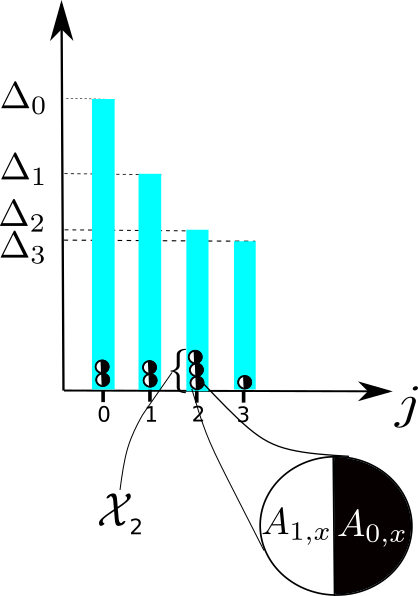
\includegraphics[width=2in]
{../uplift/uplift-bins.png}
\caption{
Pictorial
representation
of the sequence
$\{(\calx_c, \Delta_c)\}_{c=0, 1, \ldots, nc-1}$.
}
\label{fig-uplift-bins}
\end{figure}


Starting with $DS$,
UM performs the following steps.
Fig.\ref{fig-uplift-bins}
is a pictorial representation
of the quantities
that are calculated
during these steps.

\begin{enumerate}
\item Find

\beq
A_x = \{\s: x^\s \approx x\}\eeq
for each observed $x\in val(\rvx)$.
Set $A_x=\emptyset$ for unobserved $x\in val(\rvx)$.

\item Use Eq.(\ref{eq-est-ace-uplift})
to calculate $\delta_x$
for each $x\in val(\rvx)$.
Set $\delta_x=0$ if $A_x=\emptyset$.

\item Partition
the set $\{\delta_x: x\in val(\rvx)\}$
into disjoint bins. Call
$\Delta_c$  the average $\delta_x$
within bin $c$ for $c=0, 1, \ldots, nc-1$.
The class labels
$c$ should be assigned
so that the sequence of
$\Delta_c$
is monotonic and non-increasing; i.e.,

\beq
\Delta_0 \geq \Delta_{1}\geq\cdots \geq \Delta_{nc-1}
\;.
\eeq
Now calculate

\beq
\calx_c =\{ x: \delta_x \approx \Delta_c\}
\eeq
 for each $c$.
By the end of this step,
we will have calculated
$\{(\calx_c, \Delta_c)\}_{c=0, 1, \ldots, nc-1}$
from $\{(x, \delta_x)\}_{x\in val(\rvx)}$.
We will refer to the $\calx_c$
as {\bf stratum-bins}. Note that
\beqa
\Delta_c &=&\frac{1}{|\calx_c|}\sum_{x\in\calx_c}\delta_x
\\
&=&
\underbrace{\frac{1}{|\calx_c|}\sum_{x\in\calx_c}Y^1_x}_
{\displaystyle Y^1_c}
-
\underbrace{\frac{1}{|\calx_c|}\sum_{x\in\calx_c}Y^0_x}_
{\displaystyle Y^0_c}
\;.
\label{eq-Delta-c}
\eeqa
\item
For each $c$,
calculate

\beq
A_{x,d}=\{\s\in A_x: d^\s = d\}
\eeq

\beq
\Sigma_{d,c}=\cup_{x\in \calx_c}A_{x,d}
\eeq
for $d\in\bool$
and

\beq
\Sigma_{c}=\Sigma_{0,c}
\cup \Sigma_{1,j}
\;.
\eeq
\end{enumerate}


\begin{figure}[h!]
\centering
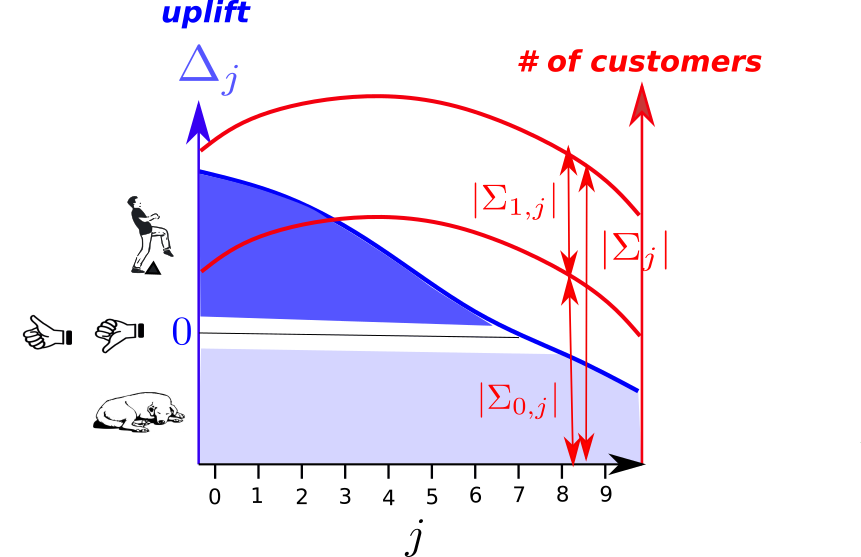
\includegraphics[width=4in]
{../uplift/qini-fake.png}

\caption{
Plot
of UM results.
}
\label{fig-qini-fake}
\end{figure}
Fig.\ref{fig-qini-fake}
is a  way of
plotting
the results
of UM in an
intuitive
way.


Another common plot of UM results is
called a {\bf Qini
curve}.
A Qini curve is a plot
of $(X_c,Y_c)$
for all $c$, where

\beq
X_c= \sum_{c'=0}^{c}\sum_{x\in \calx_{c'}}|A_x|
\eeq
is the cumulative population (counting the
samples in
order of decreasing uplift) and

\beq
Y_c=\sum_{c'=0}^c \Delta_{c'}
\eeq
is the cumulative uplift.
As $c$ increases, a Qini curve rises fast at first and then its slope decreases until
at some value $c_0$, the slope is defined as too small to care. No marketing resources are
directed towards
participants $\s$ for whom  $c>c_0$.\footnote{
Let
$S_{\Delta} = \{\s:\delta^\s \geq \Delta\}$.
A Qini curve can also be defined, without stratification,
as a
 plot of $(X_\Delta, Y_\Delta)$ for all $\Delta>0$,
where $
X_\Delta = |S_{\Delta}|$
and
$
Y_\Delta= \sum_{\s\in S_{\Delta}}\delta^\s
$. As $\Delta$ decreases, a Qini curve rises fast at first and then its slope decreases.
}

\section{Trees}

Generic dtrees are
described in Chapter \ref{ch-dtree}.
In the discussion below, we will assume that the reader has read
that chapter already.

For our previous discussion,
we assumed a dataset
$DS= \{ (\s, d^\s, x^\s, y^\s):
 \s\in\Sigma\}$ and
 assumed we had a stratifying
 method to obtain the stratum
 $c^\s$ of each sample $\s$.
In this section, we will assume
from the onset an
extended dataset
$DS^+= \{ (\s, c^\s, d^\s, x^\s, y^\s):
 \s\in\Sigma\}$
that contains the stratum $c^\s$ for each sample $\s$.
This extended dataset will be used
to train a dtree to find the stratum of
a sample. Thus, the dtree will
do the job of the prior stratifying method.

Next,
let us describe how to
modify the results
of Chapter \ref{ch-dtree}
on generic dtrees
to the case of UM dtrees.
The main difference,
as we will
explain in detail
next,
is that we use two dtrees ($d=0,1$) instead
of one. Each dtree reduces to a LD bnet. The two
bnets have the same structure but
different branch probabilities.
Furthermore, instead of the Information
Gain metric
used for generic dtrees,
we use a different
metric, one
that connects the branch probabilities
of the twin bnets.

For UM, we consider two dtrees,
labeled by the treatment dose $d=0,1$ (no dose, dose).
For each $d$, let $N_j^d(c, x_j)$ be the number
of individuals $\s$
in the population that is exiting question node $j$,
belonging to class $c$ and having $\rvx_j=x_j$.
From $N_j^d(c, x_j)$, we can define
an empirical
probability distribution

\beq
P(c, d, x_j|j)
=
\frac{N_j^d(c, x_j)}{N_j}
\;,\;\; \text{ where }
N_j=\sum_{c, d, x_j}N_j^d(c, x_j)
\eeq
Once
we have an empirical probability distribution
$P(c, d, x_j| j)$ for each node $\rvx_j$ and
class $c$,
we can define various conditional
probabilities, and from those
conditional probabilities,
we can define various metrics.



In Chapter
\ref{ch-dtree},
we used Information
Gain
(a mutual information)
as the SAM (Separation Ability Measure)
in
SL (Structure Learning)
of dtrees (Decision Trees).
Information Gain
is a bad
SAM for SL of UM dtrees,
because it knows nothing about
 $d=0,1$.
For
UM dtrees,
we need a SAM specifically
designed to separate $d=0,1$, and generate
classes that are
 uplift bins (i.e., uplift intervals).


Ref.\cite{jaros}
proposes and studies
the following
3 SAMs
for doing SL of UM dtrees.


\begin{enumerate}
\item{\bf SAM\_DD} (DD=Delta Delta)

For $d\in \bool$
and $c, c'\in val(\rvc)$, define the increments

\beq
\partial_d f(d)=f(1)-f(0)
\eeq
and

\beq
\partial_{c',c} f(c)=f(c')-f(c)
\;.
\eeq
Let

\beqa
\Delta_{c|j} &=& P(c|j,1)-P(c|j,0)
\\
&=& \partial_d P(c|j,d)
\label{eq-delta-c-j}
\eeqa

\beqa
SAM\_DD_j&=& \max_{c,c'}|\partial_{c',c}\partial_d P(c|j,d)|
\\
&=&
\max_{c,c'}|\partial_{c',c}\Delta_{c|j}|
\eeqa

\item{\bf SAM\_KL} (KL=Kullback Leibler)
\begin{align}
SAM\_KL_j&=
\left[
\sum_{x_j\in val(\rvx_j)}
P(x_j|j)
D_{KL}(P_{\rvc|x_j,j,1}\parallel P_{\rvc|x_j,j,0})
\right]
-
D_{KL}(P_{\rvc|j,1}\parallel P_{\rvc|j,0})
\\
&=\left\{\begin{array}{l}
\left[
\sum_{x_j\in val(\rvx_j)}
P(x_j|j)
 \sum_{c\in val(\rvc)}P(c|x_j,j,1)
\ln \frac{P(c|x_j,j,1) }{ P(c|x_j,j,0) }
\right]
\\
-
\sum_{c\in val(\rvc)}
P(c|j,1)
\ln \frac{P(c|j,1) }{ P(c|j,0) }
\end{array}
\right.
\label{eq-sam-kl}
\end{align}

{\bf $SAM\_KL_j$ can be negative.}

\item {\bf SAM\_E} (E=Euclidean)

$SAM\_E_j$ is defined the same way as $SAM\_KL_j$
except with
the KL divergence $D_{KL}(P\parallel Q)$
in $SAM\_KL$ replaced
by the Euclidean distance squared.


\beq
D(P,Q) =\sum_x (P(x)-Q(x))^2
\eeq

\end{enumerate}

The intuitive reason for
 using these quantities as
SAMs is that they maximize the change in uplift
between
successive tree levels, so
that the uplift increases as quickly as possible
as we descend down the UM tree.
In the case of generic dtrees
for which we use Information Gain as SAM, we
are maximizing the correlation
between classes and nodes as we descend down the tree.
These two goals are related.
In fact, in the limit
where the
number of control individuals
becomes zero,
$SAM\_KL_j$ and $IG_j$
become the same, as will be shown later.

Next we show
that $SAM\_KL_j$
satisfies the following 3
axioms\footnote{
We won't show it
here, but
according to Ref.\cite{jaros},
$SAM\_E_j$ also satisfies these
3 axioms, but
$SAM\_DD_j$
satisfies only the first two.}

\begin{claim}
.\newline
\begin{enumerate}
\item \label{item-sam-min}
$SAM\_KL_j$
is minimum
iff
$P(c|x_j,j,0)=P(c|x_j, j,1)$
for all $c$ and $x_j$.
\item \label{item-sam-zero}
If $P(c|j,d)=P(c|d)$
for all $c,d$, then $SAM\_KL_j=0$.
\item
\label{item-no-control}
Suppose $N(d=0)=0$ for all nodes $r\in J_0$
 (i.e., no control population)
and we use the Laplace Correction
when warranted. Then

\begin{align}
SAM\_KL_j
&=
H(\rvc:\rvx_j|j,1)
\\
&=
IG_j\;\;\; \text{ for treated population}
\;.
\end{align}
\end{enumerate}
\end{claim}
\proof

The proof of items
\ref{item-sam-min}
and \ref{item-sam-zero}
follow by inspection of Eq.(\ref{eq-sam-kl}).
Item \ref{item-no-control}
is proven in Claim \ref{claim-no-control}
below.
\qed



Let $N_\rvc=|val(\rvc)|$.
Define the uniform probability
distribution

\beq
U_\rvc(c)=\frac{1}{N_\rvc}
\eeq
for all $c\in val(\rvc)$.

Empirical
probabilities that are undefined
when $N_j^d=0$ can be
\qt{Laplace Corrected}
as follows:

\beq
P(c|j,d)=
\left\{
\begin{array}{ll}
\frac{N_j^d(c)}
{N_j^d}&\text{ if } N_j^d>0
\\
U_\rvc(c) & \text{ if $N_j^d=0$ (Laplace Correction)}
\end{array}
\right.
\eeq




\begin{claim}
\label{claim-no-control}
Suppose $N_r(0)=0$ for all dtree nodes $r\in J_0$
and we use the Laplace Correction
when warranted. Then

\beq
SAM\_KL_j=H(\rvc:\rvx_j|j,1)
\;.
\eeq
\end{claim}
\proof

For all nodes $r\in J_0$, we  must have

\beq
P_{\rvc|r,0}=U_\rvc
\eeq
so

\beqa
D_{KL}(P_{\rvc|r,1}\parallel P_{\rvc|r,0})
&=&
D_{KL}(P_{\rvc|r,1}\parallel U_\rvc)
\\
&=&
\ln(N_\rvc) - H(\rvc|r,1)
\;.
\label{eq-kl-reduce}
\eeqa
For all $x_j\in val(\rvx_j)$, we must also have


\beq
N_j=N_j^1, \quad N_j(x_j)=N_j^1(x_j)
\eeq
so

\beq
P(x_j|j)=
P(x_j|j,1)
\;.
\label{eq-p-kj-add-1}
\eeq
Now using Eqs.(\ref{eq-kl-reduce}) and
 (\ref{eq-p-kj-add-1}), we get


\beqa
SAM\_KL_j&=&
-\left[
\sum_{x_j\in val(\rvx_j)}
P(x_j|j)
H(\rvc|x_j,j,1)
\right]
+
H(\rvc|j,1)
\\
&=&
-\left[
\sum_{x_j\in val(\rvx_j)}
P(x_j|j,1)
H(\rvc|x_j,j,1)
\right]
+
H(\rvc|j,1)
\\
&=&
-H(\rvc|\rvx_j,j,1)+H(\rvc|j,1)
\\
&=&
H(\rvc:\rvx_j|j,1)
\eeqa
\qed

\hrule\noindent
{\bf Connection between
$\Delta_c$
and $\Delta_{c|j}$}

Recall Eq.(\ref{eq-Delta-c}):

\beqa
\Delta_c &=&
\underbrace{\frac{1}{|\calx_c|}\sum_{x\in\calx_c}Y^1_x}_
{\displaystyle Y^1_c}
-
\underbrace{\frac{1}{|\calx_c|}\sum_{x\in\calx_c}Y^0_x}_
{\displaystyle Y^0_c}
\\
&=&
\partial_d Y^d_c
\;.
\eeqa
Compare that to Eq.(\ref{eq-delta-c-j}):
\beqa
\Delta_{c|j} &=& P(c|j,1)-P(c|j,0)
\\
&=& \partial_d P(c|j,d)
\eeqa
What is the connection
between these 2 deltas, $\Delta_c$
and $\Delta_{c|j}$? Are they equal?

First off, notice that
$\Delta_{c|j}$ is defined for all
nodes $j$ of the dtree. Let
$j(c)$ be the leaf node
for which $\Delta_c\approx \Delta_{c|j(c)}$.
Assume $y^\s\in\bool$. Then

\beq
P(c|j=j(c), d)=\frac{N^d_{j(c)}(c)}{N^d_{j(c)}}
\approx Y^d_c
\eeq
So the two deltas are indeed approximately equal
when $y^\s\in \bool$ and $j=j(c)$.

\end{document}
